\documentclass[14pt]{extarticle}
\usepackage{extsizes}
\usepackage{geometry}
\geometry{margin=0.5in}

%% for images
\usepackage{graphicx}
\graphicspath{ {images/} }

%% language support
\usepackage[T1,T2A]{fontenc}
\usepackage[utf8]{inputenc}
\usepackage[english,russian]{babel}

\usepackage{amsmath}
\usepackage{tikz}

%% hyperrefs
\usepackage{hyperref}
\hypersetup{
    colorlinks,
    citecolor=black,
    filecolor=black,
    linkcolor=black,
    urlcolor=black
}

\title{2024}
\author{КЫК}
\begin{document}
\maketitle
\tableofcontents

\section{Геометрическая оптика и её законы. Относительный и абсолютный показатель
преломления. Явление полного внутреннего отражения и его применение. Закон
обратимости световых лучей.}

\textbf{Четыре закона оптики:}
\begin{enumerate}
    \item Закон прямолинейного распространения света: 
    в однородной среде свет распространяется прямолинейно 
    \item Закон независимости световых лучей: 
    при пересечении световые лучи не возмущают друг друга
    \item Закон отражения света:
    отражённый луч лежит в одной плоскости с падающим лучом и 
    нормалью, восстановленной в точке падения. Угол падения равен 
    углу отражения. 
    \item Закон преломления света:
    преломленный луч лежит в одной плоскости с падающим лучом и нормалью,
    восстановленной в точке падения. Отношение синуса угла падения к синусу
    угла преломления есть величина постоянная для данных веществ:
    $\frac{\sin i_1}{\sin i_2} = n_{12} = const$
\end{enumerate}
Величина $n_{12}$ называется \textbf{относительным показателем преломления} 
второго вещества по отношению к первому.\\
Показатель преломления вещества по отношению к вакууму называется 
\textbf{абсолютным показателем преломления} данного вещества.\\\\
Предельный угол - такой угол падения, начиная с которого угол преломления 
равен $90^\circ$, т.е. свет не проникает во вторую среду и интенсивность
отраженного луча равна интенсивности падающего. Это явление называется
\textbf{полным внутренним отражением}.\\
Полное внутреннее отражение (т.е. отсутствие поглощения света) 
используется в волоконной оптике для передачи световых сигналов на большие
расстояния, а также в оптических приборах.\\\\
\textbf{Закон обратимости световых лучей:} если навстречу лучу, 
претерпевшему ряд отражений и преломлений, пустить другой луч, то 
он пойдет по тому же пути, что и первый (прямой) луч, но в 
обратном направлении. 

\section{Прохождение света через призму. Вывод угла отклонения при прохождении света
через призму с малым углом преломления}
Coming soon.
\section{Геометрическая оптика. Принцип Гюйгенса. Связь 
абсолютного показателя
преломления со скоростью распространения света в среде.}

\textbf{Принцип Гюйгенса:} каждая точка, до которой доходит
волновое движение, служит центром вторичных волн; огибающая
этих волн даёт положение фронта волны в следующий момент. 
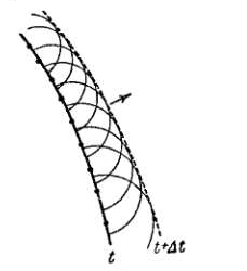
\includegraphics{wavefront.png}
Абсолютный показатель преломления $n$ и скорость распространения 
света в среде $v$ связаны соотношением: $n = \frac{c}{v}$, 
получаемым из волновой теории.
\\
\section{Световой поток. Кривая видности. Точечный источник.
Сила света и световой поток:
определения и единицы измерения}
\textbf{Световой поток} - поток лучистой энергии, оцениваемый
по зрительному ощущению. Полный световой поток равен 
$\Phi = \int_{0}^{\infty} V(\lambda) \phi(\lambda) d\lambda$,
где $V(\lambda)$ - функция видности, $\phi(\lambda)$ - 
функция распределения энергии потока по длинам волн, 
$\lambda$ - длина волны.\\
\textbf{Кривая видности} даёт чувствительность среднего нормального
человеческого глаза к излучению разной длины волны:
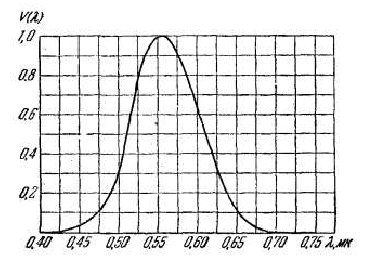
\includegraphics{visibility_curve.png} 
Как видно, максимум на длине волны 0.555 мк (зеленая часть спектра).
\\\\
\textbf{Точечный источник} - такой источник света, размерами
которого можно пренебречь по сравнению с расстоянием от места
наблюдения до источника.\\
\textbf{Сила света} - поток излучения точечного источника, 
приходящийся на единицу телесного угла: 
$I = \frac{d\Phi}{d\Omega}$. Единица измерения - свеча (св).\\
Единица измерения светового потока - люмен (лм).
1 лм = 1 св * 1 стер.
\section{Световой поток. Кривая видности. Освещенность, светимость, яркость: определения и
единицы измерения.}
\textbf{Освещенность} - характеризует степень освещенности 
поверхности падающим на неё световым потоком: 
$E = \frac{d\Phi_{пад}}{dS}$. Единица измерения освещенности - 
люкс (лк), 1лк = 1 лм : 1 $м^2$.\\
\textbf{Светимость} - световой поток, испускаемый единицей 
поверхности наружу по всем направлениям: 
$R = \frac{d\Phi_{исп}}{dS}$. Измеряется также в люксах. 
\section{Принцип Ферма. Оптическая длина пути. Вывод из принципа Ферма закона
отражения.}
\textbf{Принцип Ферма} - свет распространяется по такому пути,
для прохождения которого ему требуется минимальное время ИЛИ 
Свет распространяется по такому пути, оптическая длина которого 
минимальна. 
\textbf{Оптическая длина пути} - величина 
$L = \int_{1}^{2} n ds$, где n - показатель преломления 
среды, $ds$ - длина элементарного отрезка пути.
\section{Принцип Ферма. Оптическая длина пути. Вывод из принципа Ферма закона
преломления.} 
Тут будут выводы.
\section{Геометрическая оптика. Основные понятия и определения: гомоцентрический и
астигматический пучок; стигматическое, действительное и мнимое изображение,
идеальная оптическая система, пространство предметов и пространство изображений.}
\textbf{Геометрическая (лучевая) оптика} - раздел оптики,
основывающийся на представлениях о световых лучах.\\
\textbf{Пучок} - совокупность лучей.\\
\textbf{Гомоцентрический пучок} - продолжения лучей 
пересекаются в одной точке. Ему соответствует сферическая
волновая поверхность. 
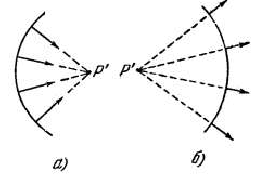
\includegraphics{beam_of_rays.png}
\textbf{Астигматический пучок} - пучок, которому соответствует
волновая поверхность двоякой кривизны. Лучи пересекаются
в совокупности точек, расположенных на двух взаимно перпендикулярных
отрезках.
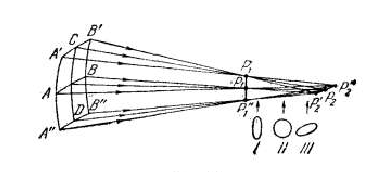
\includegraphics{beam_of_rays2.png}
Если оптическая система не нарушает гомоцентричности пучков,
то лучи, вышедшие из одной точки $P$, пересекутся также в одной
точке $P^{'}$ - \textbf{оптическом изображении} первой точки. Если 
любая точка предмета изображается в виде точки, то изображение
предмета называется \textbf{точечным (стигматическим)}.\\
Изображение \textbf{действительное}, если световые лучи 
действительно пересекаются в $P^{'}$, и \textbf{мнимое},
если в $P^{'}$ пересекаются продолжения лучей, проведенные
в направлении, обратном распространению света.\\
Оптическая система, дающая стигматическое изображение, 
геометрически подобное изображаемому предмету, называется
\textbf{идеальной}. С помощью такой системы 
пространственная непрерывность точек $P$ изображается 
в виде пространственной непрерывности точек $P^{'}$. 
Первая называется \textbf{пространством предметов}, вторая - 
\textbf{пространством изображений}.
\section{Центрированная оптическая система. Кардинальные точки и плоскости
центрированной оптической системы.}
Оптическая система, образованная сферическими (в частности
плоскими) поверхностями, называется \textbf{центрированной}, 
если центры всех поверхностей лежат на одной прямой. 
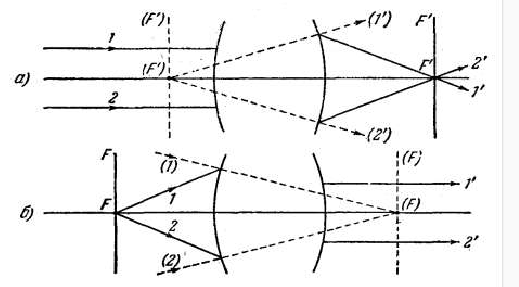
\includegraphics{optic_system.png}
\textbf{Кардинальные плоскости} - фокальные, главные и 
узловые плоскости.
\textbf{Кардинальные точки} - фокусы, главные точки и узлы.
\section{10. Центрированная оптическая система. Отражение и преломление на сферической
поверхности. Оптическая сила сферической поверхности.}
Похуй.
\section{Линза. Тонкая линза, её характерные точки и лучи. Оптическая сила. Построение
изображений в тонких линзах. Поперечное увеличение}
\textbf{Линза} - система двух сферических преломляющих 
поверхностей. 
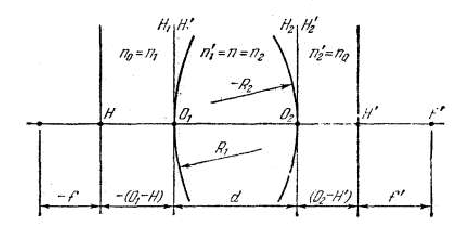
\includegraphics{lense.png}
Линза с пренебрежимо малым $d$ называется тонкой. В случае тонкой
линзы расстоянием $O_1 O_2$ можно пренебречь и считать их
находящимися в одной точке, называемой 
\textbf{оптическим центром} тонкой линзы. Любой луч, идущий
через него, не изменяет своего направления.\\
Оптическая сила тонкой линзы равна алгебраической сумме 
оптических сил преломляющих поверхностей:
$\Phi = \Phi_1 + \Phi_2$\\
\section{Вывод формулы тонкой линзы с использованием хода кардинальных параксиальных
лучей.}
\textbf{Формула тонкой линзы:} $\frac{1}{s^{'}} - 
\frac{1}{s} = \frac{n - n_0}{n_0} \bigl(\frac{1}{R_1}
-\frac{1}{R_2}\bigr)$
\section{Линза. Тонкая линза. Формула тонкой линзы. Аналитическое исследование формул
тонкой собирающей и рассеивающих линз}
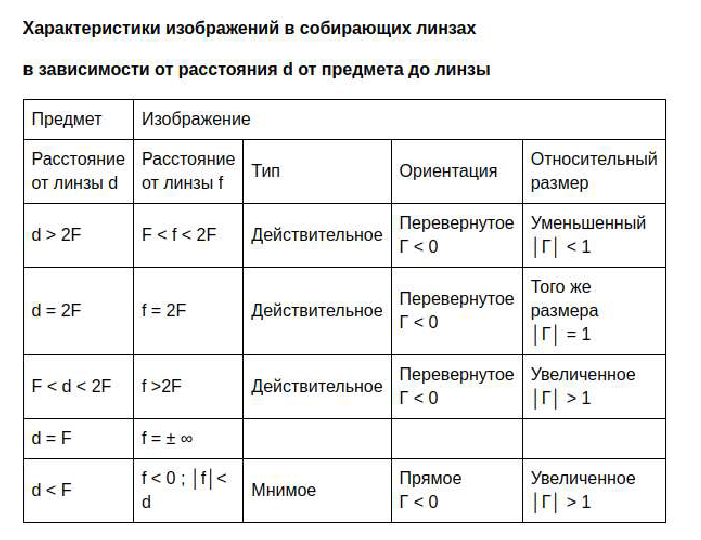
\includegraphics{lense_analysis.png}
\section{ Человеческий глаз как оптическая система (аккомодация, 
расстояния наилучшего зрения, дефекты зрения и их коррекция).}
\textbf{Аккомодация} - способность глаза менять фокусное расстояние
глаза посредством мышечного усилия, приспосабливаясь к 
расстоянию до рассматриваемого предмета. Ограничена снизу 20 см.\\
\textbf{Расстояние наилучшего зрения} - расстояние, на котором
нормальный глаз испытывает наименьшее напряжение при 
рассматривании деталей предмета.\\
\textbf{Близорукость} - дефект зрения, при отсутствии 
аккомодации изображение предмета лежит впереди сетчатки. 
Корректируется рассеивающей линзой.\\
\textbf{Дальнозоркость} - дефект зрения, при отсутствии 
аккомодации изображение предмета лежит за сетчаткой. 
Корректируется собирающей линзой.\\
\textbf{Астигматизм} - дефект зрения, искажённая кривизна 
роговицы и/или хрусталика, что провоцирует нечеткость изображения. 
Корректируется цилиндрическими линзами.\\
\section{Оптические приборы (лупа, микроскоп, зрительная труба). Увеличение прибора}
Bullshit.

\end{document}
